\documentclass[a4paper,english, 11pt]{article}

\usepackage{siunitx} 
\usepackage[hidelinks]{hyperref}
\usepackage[a4paper,inner=2.5cm,outer=2.5cm,top=2.5cm,bottom=2.5cm,pdftex]{geometry} 
\usepackage{array}
\usepackage{fancyhdr}
\usepackage{graphicx}     
\usepackage{natbib}
\usepackage{hyperref}
%\usepackage{url}
\usepackage{tcolorbox}
\usepackage{titling}
\usepackage{listings}
\usepackage{color}

\newcommand{\subtitle}[1]{%
  \posttitle{%
    \par\end{center}
    \begin{center}\large#1\end{center}
    \vskip0.5em}%
}
\newcommand{\emailme}{\href{mailto:data.nleg@unis.no}{data.nleg@unis.no}}

\definecolor{dkgreen}{rgb}{0,0.6,0}
\definecolor{gray}{rgb}{0.5,0.5,0.5}
\definecolor{mauve}{rgb}{0.58,0,0.82}

\graphicspath{{../Images/}} 
\bibliographystyle{agsm}

\title{How to publish FAIR Nansen Legacy datasets}
\subtitle{A complete step by step guide}
\date{\today\\v0.1}
\author{Luke Marsden (\emailme)}

\begin{document}
\maketitle
\tableofcontents
\pagestyle{fancy}
\newpage
\section{Introduction}
\label{s:Introduction}

Publishing your data benefits both you and the broader scientific community. It supports transparency and reproducibility of your research, and allows others to work with your data, thus promoting collaboration. Published datasets are visible and citeable, and can be included on your CV and grant applications. As outlined in both the data management plan \citep{aendmp2021} and data policy \citep{aendatapolicy2021} we are committed to publishing FAIR data \citep{wilkinson2016fair}, meaning that data should be:

\begin{itemize}
\item Findable: Data and metadata are findable by humans and computers and assigned a persistent identifier (e.g. DOI).
\item Accessible: Data and metadata can be freely and openly accessed, allowing authentication and authorization if necessary.
\item Interoperable: Data and metadata use standardised terms (common vocabularies) and file structures allowing use in different applications or workflows with minimal manual intervention. 
\item Reusable: Data and metadata are richly and clearly described for humans and computers to understand and have a clear data usage license. 
\end{itemize}

When you publish an paper in a scientific journal, it is now often a requirement that the data are published in a data repository, usually making the data findable and accessible. However, this does not necessarily mean that the data are easy for someone else to use. Here, we will go step-by-step through how to publish FAIR datasets in the Nansen Legacy project.

\section{Selecting a suitable file type and conventions}
\label{s:FileType}

The first step is to identify what type of data you are working with. This will determine what file format you should convert your data to, and which conventions should be used for the metadata. For most Nansen Legacy datasets, NetCDF-CF or DwCA should be used. See Table \ref{t:netcdf_vs_dwca} for examples. Please email \emailme if you are unsure or if you think your data are an exception.

\begin{table}[h!]
  \begin{center}
    \label{t:netcdf_vs_dwca}
    \begin{tabular}{l|r} % <-- Alignments: 1st column left, 2nd middle and 3rd right, with vertical lines in between
      \textbf{NetCDF-CF} & \textbf{DwCA}\\
      \hline
      Physical data & Biodiversity data\\
      Physical oceanography data & Ecological data\\
      Atmospheric data & Measurements of species/individual\\
      Sea water temperature & Primary production rate\\
      Particulate organic carbon in sea water & Age of fossil\\
      Wind speed & Fatty acids in fish\\
      Sea ice thickness & List of species from processed DNA data\\
      Chlorophyll A concentration & Virus diversity\\
      
    \end{tabular}
    \caption{Examples of data that should be stored as either NetCDF-CF or DwCA}
  \end{center}
\end{table}

You can refer to XXXX, a spreadsheet that lists various parameters measured in the Nansen Legacy project, and the file type, standard name and units that should be used when publishing the data. If the parameter that you are working with is missing from this spreadsheet, please contact \emailme so it can be added.

If your data should be converted to NetCDF-CF, go to section.

If your data should be converted to DwCA, go to section.

\section{NetCDF-CF}
\label{s:NetCDF-CF}

Some information first about NetCDF-CF. 

NetCDF (Network Common Data Forum) is a file format that is used for storing multidimensional scientific data in grids. There are several components of a NetCDF file. Scientific data (such as wind speed, sea water temperature etc.) are stored as 'variables', whose values are stored in a multidimensional grid. Dimensions may be for example time or a spatial coordinate.

When creating a NetCDF file, one must first define the dimensions with regular increments, thereby defining a multidimensional grid if more than one dimension is defined. The file creator then defines which dimensions the variable uses (this may not be all of them if storing more than one variable in the same file). Values must be assigned for the variable at every point in the multidimensional grid. There may be some points in the grid where a value does not exist. In these cases, a 'fill value' is defined. This fill value is a constant value that is unrealistic, e.g. orders of magnitude too high for example.

\begin{figure}[htb]
    \tcbox[colback=white]{
    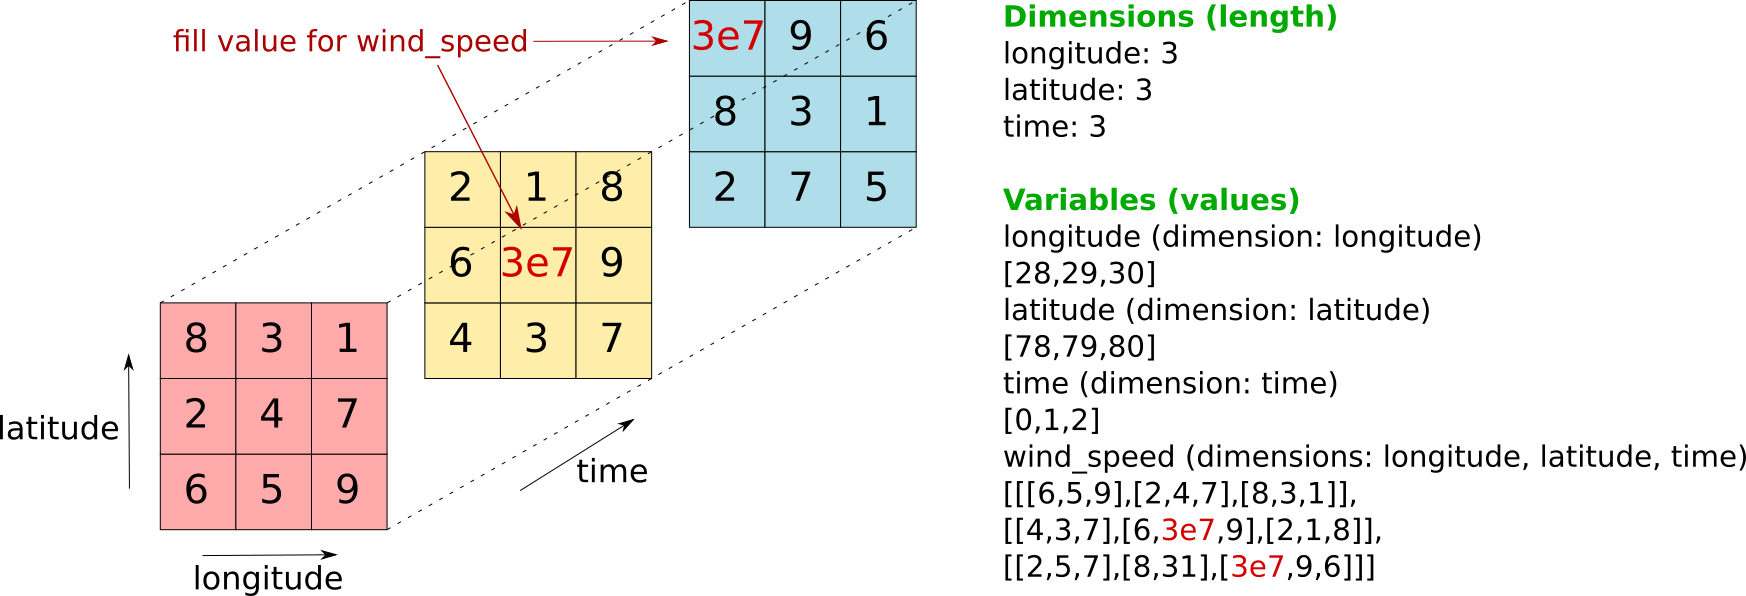
\includegraphics[width=0.93\textwidth]{netcdf.png}
    }
    \caption{\label{fig:netcdf}
        Visualisation of a multidimensional netCDF file, with 3 dimensions: longitude, latitude and time.
        Each dimension has a set length (each 3 in this case), and the values
        for the dimension are stored as a variable with the same name.
        Each variable has values defined, and references dimensions which define the 'location' of each value in the grid. The wind$\_$speed variable has 3 dimensions in this case (longitude, latitude and time). Values for the wind$\_$speed variable are plotted, and a fill value of 3e7 has been used where no measurement was taken. 
    }
\end{figure}

A NetCDF file also includes 'variable attributes' (metadata that describe each variable) and 'global attributes' (metadata that describe the file as a whole). Widely accepted conventions must be used that define the names of the attributes, which attributes to use and descriptions on how to populate them. Conventions ensure consistency between data created by different users, and make the data both human and machine readable, required for the data to be interoperable and reusable (FAIR - \ref{s:Introduction}). We reference what conventions we use as a global attribute. 

The Climate and Forecast (CF) conventions (hence NetCDF-CF) are 'use' metadata, that instruct someone on how to use the data. They define 'standard names' and units to be used for different variables, with descriptions. The official documentation for the NetCDF-CF conventions can be found here (\url{http://cfconventions.org/}).

We also use the Attribute Convention for Data and Discovery (ACDD), which are 'discovery' metadata that help someone to find the data. They define variable and global attributes that are recommended for use. We will outline which attributes to use for Nansen Legacy datasets in sections \ref{ss:globalattributes} (global attributes) and \ref{ss:variableattributes} (variable attributes). Information on ACDD can be found here (\href{https://wiki.esipfed.org/Attribute_Convention_for_Data_Discovery_1-3}{https://wiki.esipfed.org/Attribute\_Convention\_for\_Data\_Discovery\_1-3}). Please make sure that this is the latest version.

\subsection{How to structure your data collection}
\label{ss:structurecollection}

What dimensions do your data have? A single depth profile? Multiple depth profiles? A time series? Or something more complicated?

How many NetCDF files you need to create will depend on this. There are different approaches, but we advise that each NetCDF file should be as simple as possible. This might mean dividing your data into multiple small files, that can be stored in a single data collection. For example, one file for each depth profile. This approach has several advantages:

\begin{itemize}
\item Each file is easier to create.
\item Each file is easier to understand.
\item If someone is interested in only a subset of the data, they can easily access these without having to download and open the rest of the data too.
\item This approach usually requires less space than storing everything in a single file. Data in NetCDF files are stored in grids with regular intervals. A 'fill value' must be assigned for each grid point where there is a gap in the data (no value measured/recorded). It is likely that there will be more 'empty' space if more dimensions are used. 
\end{itemize}   

Consider how many files you will need to create. Consider what is constant for each file (global attributes), what varies within each file (variables and dimensions) and what varies between the different files.

If each data point corresponds to a single event in the metadata catalogue (i.e. a single row in the sample logs) the event ID should also be stored in this file, to link the metadata catalogue and data together. We will get back to how to do this later (section XX).

\subsection{Dimensions and variables: cleaning up your input data}
\label{ss:dimensionsvariables}

You should now know what your dimensions and variables will be for each file. These might correspond to individual columns in a spreadsheet or CSV file for example. You can now focus on preparing these data to make converting them to NetCDF easier.

\begin{enumerate}
\item Do you have all the columns you need?
\begin{itemize}
\item Collect all the columns you need in one file.
\item If metadata associated with your data was logged in \href{https://sios-svalbard.org/cgi-bin/darwinsheet/?setup=aen}{Nansen Legacy sample logs}, you should have corresponding Event IDs (one per data point or one per data collection in some cases). The metadata you logged are updated before they are uploaded to the \href{https://sios-svalbard.org/aen/tools}{metadata catalogue on SIOS} - cleaned and errors corrected. You can retrieve the updated metadata at REF. You will publish some of these metadata with your data. This tool also outputs event times in ISO 8601 format, necessary for publishing.    
\end{itemize}
\item Use standardized column headers
\begin{itemize}
\item Dimensions: 
TIME SINCE? DIMENSION NAMES FROM COMMON VOCABULARY?
\item Variables:
Select a standard name for each variable from \href{https://cfconventions.org/standard-names.html}{https://cfconventions.org/standard-names.html}. Use this as your column header. Pay attention to the description and units. It may be necessary to convert your data to the units listed. If no suitable standard name exists, please email \emailme.  
\end{itemize}
\item Clean each column that will be used:
\begin{itemize}
\item Don't include text in columns that should contain only numbers.
\item Make sure all values make sense (e.g. no negative volumes).
\item If no real value was measured, leave it blank or assign a fill value. This fill value should be an unrealistic value, e.g. excessively high, or negative. Use the same fill value/blank for each case in the column. Different values can be used for different variables. Make a note of this fill value - it will be provided as a variable attribute later, which we will cover in section REF.
\end{itemize}
\end{enumerate}

\subsection{Global attributes}
\label{ss:globalattributes}

Global attributes provide discovery metadata that are related to each NetCDF files as a whole. Each attribute name is taken from a common vocabulary, and has a description associated with it to help you fill it in, and to someone working with your data to understand the contents.

A list of what global attributes must be included can be found here:
\href{https://adc.met.no/node/4}{https://adc.met.no/node/4}

Here is some extra help for some of the attributes, specific to Nansen Legacy:
\begin{itemize}
\item id: This should be a universally unique ID (UUID). If a single event ID in the metadata catalogue is related to the whole file, and only that file, it can be included here. Otherwise, a different UUID must be generated. This UUID should be reproducible, in case you want to update the file. Version 5 UUIDs are generated by 'hashing a namespace identifier'. This means that they are created from text, and the text can be recovered from the UUID also. ELABORATE ON WHAT THESE ARE AND HOW TO CREATE THEM.
\item keywords: Can be selected from WHERE?
\item creator: This is the contact person for the data, who is principally responsible for the data, and who will be listed as 'authors' if the data are cited. Can be multiple people separated by commas.  
\item publisher: Provide details for the data repository where you are publishing your data. See section REF.
\item license: According to the project data policy \citep{aendatapolicy2021}, all data should be published with the Creative Common Attribution license (\href{https://creativecommons.org/licenses/by/4.0/}{https://creativecommons.org/licenses/by/4.0/}). Include this URL for the attribute value. 
\item acknowledgements: Refer to the Research Council of Norway who fund the project, and anyone involved in recorded, analysing or processing the data up to this point.
\end{itemize}

Additional global attributes can also be included, defined by the user. Make sure that the attribute names you select are understandable, . In the Nansen Legacy project, we recommend also including the following global attributes are included as a minimum. 

\begin{itemize}
\item sampling$\_$protocols: Cite the published Nansen Legacy sampling protocols. Remember to refer to a specific version and section within.
\item depth$\_$of$\_$seabed$\_$in$\_$meters: Can be taken from the 'Bottom depth in meters' column in the metadata catalogue.
\item metadata$\_$link: DOI provided for the file by the data repository.
\end{itemize}   

Make sure you have all of this information before you proceed to section \ref{ss:convertingnetcdf}.

\subsection{Variable attributes}
\label{ss:variableattributes}

Variable attributes provide metadata that describe each variable. A list of variable attributes can be found at \url{https://wiki.esipfed.org/Attribute_Convention_for_Data_Discovery_1-3}, and we recommend that all the 'highly recommended variable attributes' are used.

Notes:
\begin{itemize}
\item The standard$\_$name is taken from the CF conventions (\url{https://cfconventions.org/standard-names.html})
\item You should convert your variable to the units stated by the standard$\_$name in the CF conventions.
\item If a suitable standard$\_$name does not exist, please contact \emailme . By liaising with the standards body, a new standard$\_$name can be proposed and added. Expanding existing standards benefits the broader scientific community.
\item The long$\_$name is not necessarily the description provided for the standard$\_$name. You can also add anything else that you think is relevant and would be useful for the data user to know.  
\end{itemize}

Make sure you have all of this information before you proceed to section \ref{ss:convertingnetcdf}.

\subsection{Converting to NetCDF-CF}
\label{ss:convertingnetcdf}

Your input data should now be ready to convert to NetCDF-CF. There a different ways to do this, depending on your data and your experience.

\begin{itemize}
\item Rosetta (\href{http://tomcat.nersc.no/rosetta/}{http://tomcat.nersc.no/rosetta/})
\begin{itemize}
\item Creating NetCDF-CF files with a simple graphical user interface. 
\item Does not require any coding experience.
\item Suitable for tabular data.
\item Not suitable for creating data with lots of dimensions.
\item Inefficient if you plan to create a large number of similar files (e.g. a large number of depth profiles).
\item To proceed with this option, go to section \ref{ss:Rosetta}.
\end{itemize}
\item Writing a script
\begin{itemize}
\item Can write a single script to create all your files (time efficient). 
\item Reusable with small tweaks for similar files in the future.
\item More control (not restricted by what Rosetta allows).
\item Learning curve if you don't code often.
\item Python (netCDF4 or xarray libraries) - introduced in section \ref{ss:xarray}
\item R - introduced in section \ref{ss:R}
\item MATLAB, Fortran...   
\end{itemize}
\end{itemize}

\subsubsection{Rosetta}
\label{ss:Rosetta}

For people who don't like to code, Rosetta provides a graphical user interface where you can create NetCDF-CF files.

\href{http://tomcat.nersc.no/rosetta/}{http://tomcat.nersc.no/rosetta/}

One disadvantage is that this approach takes a long time if you have lots of similar files. Also, it can be more difficult to create complex multidimensional files. However, for simple files, it can be very effective and easy to learn.

\subsubsection{Creating NetCDF-CF files in Python using xarray}
\label{ss:xarray}

Examples on how to convert data to NetCDF-CF using xarray can be found on GitHub at \href{https://github.com/SIOS-Svalbard/AeN_doc}{https://github.com/SIOS-Svalbard/AeN\_doc}. These examples include:

ADD HYPERLINKS

\begin{itemize}
\item{Depth profiles at a single location}
\item{A time series of data} 
\item{Multidimensional data}
\end{itemize}



More useful information can be found in these locations:
\begin{itemize}
\item \href{http://xarray.pydata.org/en/stable/generated/xarray.Dataset.html}{http://xarray.pydata.org/en/stable/generated/xarray.Dataset.html}
\item \href{https://rabernat.github.io/research_computing_2018/xarray.html}{https://rabernat.github.io/research\_computing\_2018/xarray.html}
\end{itemize}


\subsubsection{Creating NetCDF-CF files in R}
\label{ss:R}


\section{Darwin Core Archive}
\label{s:DwCA}

\section{Making data available via SIOS}
\label{s:SIOS}

According to the Nansen Legacy data policy \citep{aendatapolicy2021}, all project data will be available via Svalbard Integrated Arctic Earth Observing System (SIOS). SIOS host a portal that provides single access point to data collected in and around Svalbard (\href{https://sios-svalbard.org/metsis/search}{https://sios-svalbard.org/metsis/search}).
Note that no data are stored with SIOS. Instead, SIOS provides links to datasets stored with contributing data repositories (Section \ref{s:repository}). 

To make your data available via SIOS, you must select a contributing data repository and email me \emailme to let me know where it has been published. Depending on the data repository, harvesting the data into SIOS happens automatically or requires some work on our side. If the data repository allows, you must also request that they tag the data with "AeN" so that one can filter using the project name when searching for datasets in SIOS. One can isolate Nansen Legacy datasets by filtering by the collection \textit{AeN} \\ 
(\href{https://sios-svalbard.org/metsis/search?f%5B0%5D=collection%3AAeN}{https://sios-svalbard.org/metsis/search?f\%5B0\%5D=collection\%3AAeN}). 
Therefore, one can easily access all the data collected across the project from a single place.  

\section{Selecting a data repository}
\label{s:repository}

There are a number of data repositories that contribute to SIOS. Which one you submit your data to depends on the type of data. There are likely a number of applicable options to choose from.

\begin{center}
\begin{tabular}{ |c|c|c|c|c| } 
\hline
Name & Link & Contact & Automatic tagging for AeN? & Type of data  \\
\hline
NIRD research data archive & \href{https://archive.norstore.no/}{https://archive.norstore.no/} & & & \\  
\hline
NMDC & \href{https://www.nmdc.no}{https://www.nmdc.no} & & & \\   
\hline
NPI & \href{https://data.npolar.no/home/}{https://data.npolar.no/home/} & & & \\   
\hline
NorDataNet & \href{https://www.nordatanet.no/}{https://www.nordatanet.no/} & & & \\   
\hline
MET & \href{https://adc.met.no/}{https://adc.met.no/} & & & \\   
\hline
\end{tabular}
\end{center}
 
\section{Getting a DOI}
\label{s:doi}




%1. Preparing data for publication
%2. Retrieving metadata from metadata catalogue
%3. What type of data is it?
%
%NetCDF - 4. What is NetCDF-CF
%NetCDF - 5. Identfying standard name, and global attributes conventions
%NetCDF - 5. NetCDF - what are the dimensions?
%NetCDF - 6. NetCDF - what tools can be used based on dimensions
%7. Overview of each method
%
%
%DwCA - 4. What is DwCA
%5. Identifying field names and other coventions
%6. Introduction to IPT
%7. Other methods for creating DwCA?
%
%8. Publishing in repository, tagging with AeN.
%9. If DwCA, publishing via IPT and other repo to harvest into SIOS
%
%Write like "If it is DwCA, click here to find out how to publish your data with GBIF and a second repository that can be harvested into SIOS using the same DOI".

\bibliography{ref} 


\end{document} 